\documentclass{sciposter}
\usepackage{lipsum}
\usepackage{listings}
\usepackage{epsfig}
\usepackage[dvipsnames]{xcolor}
\usepackage{amsmath}
\usepackage{amssymb}
\usepackage{multicol}
\usepackage{graphicx,url}
\usepackage[portuges, brazil]{babel}   
\usepackage[utf8]{inputenc}

\newtheorem{Def}{Definition}


\title{\Huge \texttt{{\color{NavyBlue}XI SEMANA UNIFICADA DE APRESENTAÇÕES}}}

\author{Caroline B. do E. Santo, Mahaira S. de Souza, Thiago de S. Messias}

\institute{\texttt{{\bf{\color{orange} 8 a 12 de Junho de 2015\\
Bacharelado em Ciência da Computação – Código: BCC\_PI\_III\_N\_G01}}}}

\leftlogo[1]{Senac-logo}

\begin{document}

\conference{{\bf PI III}- Senac, 25 de Maio de 2015, São Paulo, Brasil}


\maketitle

\bf{\hrulefill}
\\
\center{
{\bf{\huge{Air Drums}}}}
\begin{multicols}{3}


\section {Resumo}

De acordo com o proposto na disciplina Projeto Integrador III, a partir do estudo e aplicação de algoritmos relacionados a visão computacional, indiretamente através da biblioteca multiplataforma OPENCV[1], foi desenvolvido o AirDrums, uma bateria em forma de jogo, onde o jogador deve seguir uma sequencia de passos para tocar a música e passar de fase, para isso, foi utilizada a biblioteca gráfica allegro 5[2] e a linguagem de programação C-99. HSV, e ponto médio foram os principais algoritmos para obter os resultados desejados.

\section{Introducão}
Nos dias atuais, é comum visualizar pessoas tocando instrumentos no ar, pratica conhecida como Air (nome do instrumento musical), desta forma originou-se o jogo AirDrums, onde o intuito é proporcionar diversão de forma rápida e fácil, via visão computacional, ou seja, não é necessário a compra de uma bateria, o jogador pode utilizar uma caneta, lápis, baquetas e etc. \\
Criado em linguagem C[3], utilizando a biblioteca gráfica allegro 5, e realizado aplicações de algoritmos em visão computacional, como HSV[4] e Ponto Médio[5], AirDrums é um jogo, cujo o objetivo é acertar os alvos que caem em cascata para arrematar pontos ao final da música. \\
Veja neste artigo, como foram aplicados os algoritmos de visão computacional e formulação das matrizes do jogo. 

\section{Revisão de Literatura}
Atualmente no mercado, existe uma diversidade de jogos envolvendo música, porém, individualmente, cada um, com sua linha de raciocínio e tecnologias.
Pensando em jogos que fizeram sucesso, temos o GuitarHero[6] e o Rock Band[7] no topo do ranking, onde em ambos, com uma guitarra o jogador precisa acertar uma sequência de notas musicais, que caiem como cascata. No Rock Band, o diferencial, é que outros instrumentos musicais são inclusos, como por exemplo a bateria.
Como simulador de instrumentos musicais, o GarageBand[8] é uma ferramenta que permite simulações de instrumentos, sem dispor do físico, é totalmente virtual. 
E a grande diferença entre o AirDrums e os jogos citados acima, é a visão computacional, possibilitando a jogabilidade sem possuir o instrumento, utilizando somente as baquetas.

\section{Desenvolvimento}

\textbf{Conversão para HSV} é a abreviação para Hue (Matriz), Saturation (Saturação), e value (Valor). \\ \\
A imagem abaixo mostra como este sistema de cores funciona. Matriz define a tonalidade, Saturação a pureza da imagem, quando mais alto o valor de saturação mais pura a imagem será, o valor define a intensidade do brilho.

\begin{figure}[!htb]
\centering
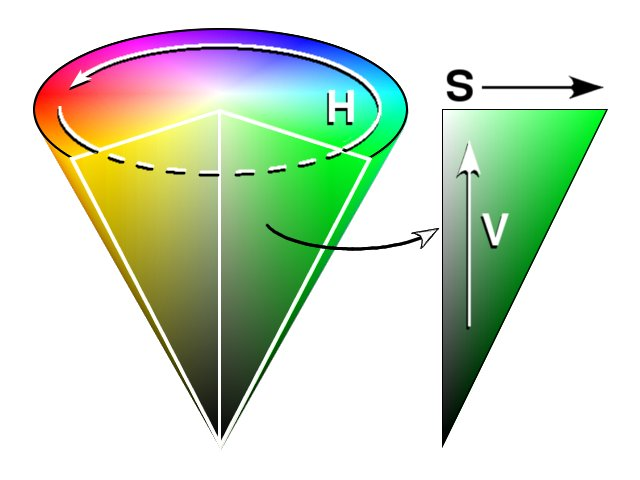
\includegraphics[scale=0.6]{HSV_cone.jpg}
\caption{Exemplo: HSV}
\end{figure}

Cada segundo da música equivale a uma matriz 4x4, desta forma o alvo aparece na posição da matriz com o elemento "1", ignorando o elemento "0", assim como mostra o exemplo abaixo
\\
\\

$ Exemplo =\left[\begin{array}{rrrr}
0 & 0 & 0 & 0\\
0 & 0 & 1 & 0\\
0 & 1 & 0 & 1\\
1 & 0 & 0 & 0
\end{array}\right],\quad$

\begin{figure}[!htb]
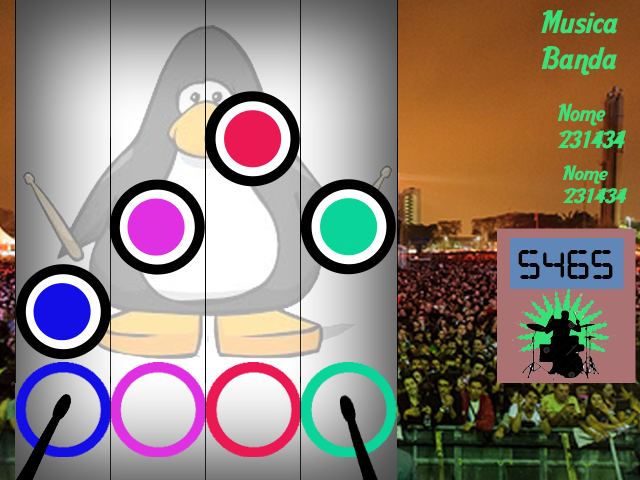
\includegraphics[width=20cm]{Exemple.png}
\caption{Alvos com posições de acordo com a matriz}
\label{alvos}
\end{figure}


\textbf{Ponto médio}[7] é o centro geométrico, ou seja o centro da massa, no jogo ele calcula o valor médio da ponta das baquetas, para que seja possível verificar o movimento que o jogador estará executando, ou seja, para cada pixel é calculado a altura do elemento x, e do elemento y, desta forma obtemos o ponto médio.

\begin{figure}[!htb]
\caption{O círculo no meio representa o ponto médio}
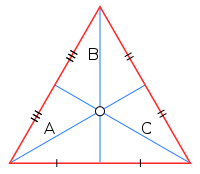
\includegraphics[width=15cm]{cent.png}
\label{Ponto médio}
\end{figure}


\section{Resultados }

Verificando os resultados, podemos chegar as seguintes conclusão:

\begin{figure}[!htb]
\centering
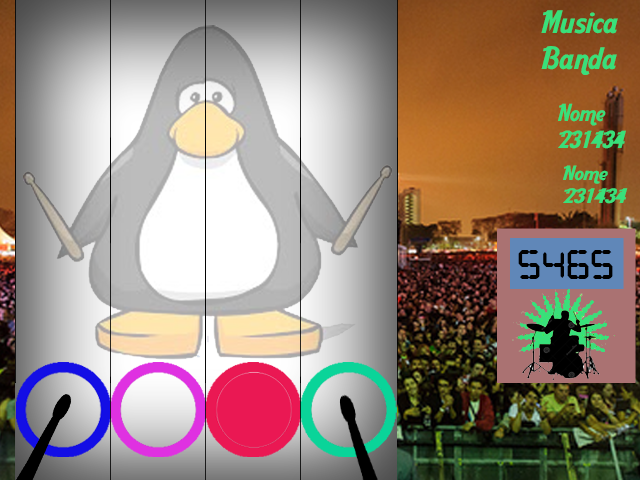
\includegraphics[scale=2.3]{AccertCase.png}
\caption{Exemplo: Caso acerte o alvo}
\end{figure}

Ao acertar o alvo, ele ficará preenchido com a cor correspondente  Assim como a imagem acima, porém se o jogador não conseguir ser rápido o suficiente para conseguir acertá-lo ao invés do alvo ser preenchido com a cor correspondente, aparecerá uma caveira para o usuário saber que está perdendo pontos, assim como podemos observar na imagem abaixo:



\begin{figure}[!htb]
\centering
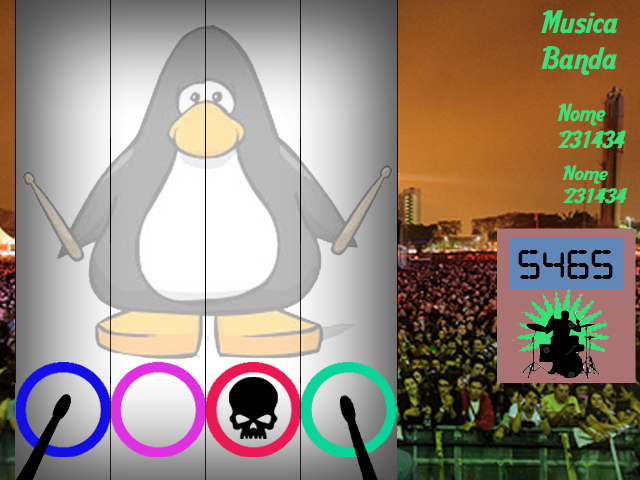
\includegraphics[scale=2.3]{ErrorCase.png}
\caption{Exemplo: Erro de alvo}
\end{figure}

\begin{figure}[!htb]
\centering
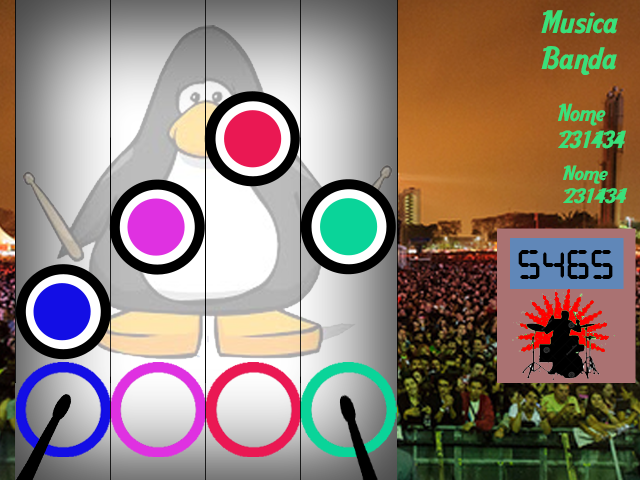
\includegraphics[scale=2.3]{BadCase.png}
\caption{Exemplo: dificuldade grande}
\end{figure}
Os alvos podem aparecer em variadas velocidades, acima temos um exemplo de alta velocidade, já a imagem abaixo mostra menor dificuldade, pois existem menos alvos caindo em cascata.

\begin{figure}[!htb]
\centering
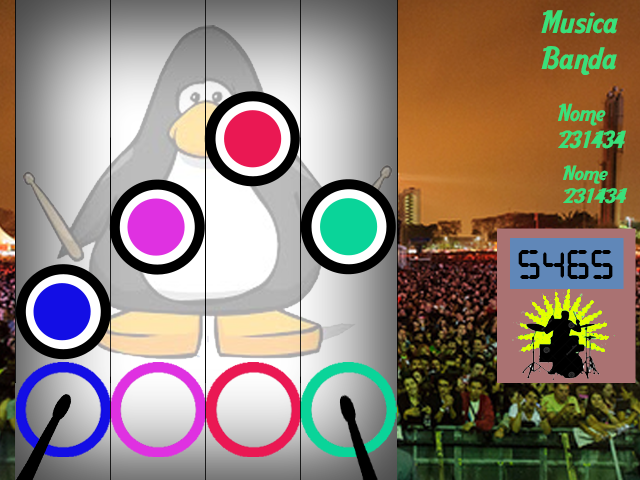
\includegraphics[scale=2.3]{mediumCase.png}
\caption{Exemplo: Nível Facil}
\end{figure}


\section{Considerações Finais}
Levando-se em conta o que foi observado, e obtido como resultado ao decorrer do projeto, podemos afirmar que o rastreamento foi a maior dificuldade em relação ao desenvolvimento, pois os algoritmos não foram triviais e alguns fatores atrapalharam, como por exemplo a iluminação do ambiente. 


\bibliographystyle{plain}
\begin{thebibliography}{9}

\bibitem{site OpenCV}
http://opencv.org/ \\
\newblock OpenCV

\bibitem{site allegro} http://www.rafaeltoledo.net/tutoriais-allegro-5/ \\
\newblock Allegro 5.

\bibitem{livro}
H. M. Deitel e P. J. Deitel.
\newblock Como programar em C, 2º edição.

\bibitem *http://sidigicor.blogspot.com.br/2011/02/modelo-hsv.html \\
\newblok Explicação do Sistema de Cores HSV

\bibitem *https://fenix.tecnico.ulisboa.pt/downloadFile/3779571421642/EstaticArq\_07\_III.pdf \\
\newblock {Centróide}

\bibitem *https://www.guitarhero.com/pt/ \\
\newblock {GuitarHero}

\bibitem *http://www.harmonixmusic.com/games/rock-band/ \\
\newblock{RockBand}

\bibitem *https://www.apple.com/br/ios/garageband/ \\
\newblock {GarageBand}
\end{thebibliography}

\end{multicols}

\end{document}